
% This LaTeX was auto-generated from MATLAB code.
% To make changes, update the MATLAB code and republish this document.

\documentclass{article}
\usepackage{graphicx}
\usepackage{color}

\sloppy
\definecolor{lightgray}{gray}{0.5}
\setlength{\parindent}{0pt}

\begin{document}

    
    \begin{verbatim}
clc, clear
close all

[rcm, Icm] = aquaMassProps();

%rcm = rcm.*100

[A,Icm_prime] = eig(Icm);


rcm_prime = A.'*rcm.';


% Random ICs

x0_deg = [-7, 2, 5].';
x0 = x0_deg*pi/180;
Tfinal = 120;

genPlots(Icm_prime, 'random')

x0_deg = [10, 0, 0].';
x0 = x0_deg*pi/180;
Tfinal = 120;

genPlots(Icm_prime, 'principal')


function genPlots(Icm_prime, name)

    load_system("eulerPropagate")

    sim("eulerPropagate")

    om = om_p;

    n = size(t,1);

    Tvec = zeros([n 1]);
    Lvec = zeros([n 3]);
    for i=1:n
        Lvec(i,:) = Icm_prime*om(i,:).';
        Tvec(i) = 0.5*dot(om(i,:).', Lvec(i,:).');
    end

    L = vecnorm(Lvec,2,2);

    T = Tvec(1);
    L = L(1);


    % Integration
    figure
    hold on
    plot(t, om(:,1))
    plot(t, om(:,2))
    plot(t, om(:,3))
    hold off

    % Energy and Momentum Ellipsoids
    Ix = Icm_prime(1,1);
    Iy = Icm_prime(2,2);
    Iz = Icm_prime(3,3);
    % Energy and Momentum Ellipsoids
    a_energy = sqrt(2*T/Ix);
    b_energy = sqrt(2*T/Iy);
    c_energy = sqrt(2*T/Iz);
    n = 100;

    x = linspace(-a_energy, a_energy, n);
    X = meshgrid(x);
    Y = zeros(size(X));
    Z = zeros(size(X));
    yu = real( sqrt((1/Iy).*(2*T - Ix.*x.^2)) );
    yl = -yu;
    for i=1:length(x)
        xi = X(:,i).';
        yi = linspace(yl(i), yu(i), n);
        Y(:,i) = yi;
        zi = real(sqrt((1/Iz).*(2*T - Ix.*xi.^2 - Iy.*yi.^2)));
        Z(:,i) = zi;
    end


    figure
    surface(X,Y,Z,'FaceColor', 'g', 'HandleVisibility', 'off')
    surface(X,Y,-Z, 'FaceColor', 'g', 'DisplayName', 'Energy Ellispoid')
    hold on

    a_mom = L/Ix;
    b_mom = L/Iy;
    c_mom = L/Iz;

    x = linspace(-a_mom, a_mom, n);
    X = meshgrid(x);
    Y = zeros(size(X));
    Z = zeros(size(X));
    yu = sqrt((1/Iy^2).*(L^2 - Ix^2.*x.^2));
    yl = -yu;
    for i=1:length(x)
        xi = X(:,i).';
        yi = linspace(yl(i), yu(i), n);
        Y(:,i) = yi;
        zi = real(sqrt((1/Iz^2).*(L^2 - Ix^2.*xi.^2 - Iy^2.*yi.^2)));
        Z(:,i) = zi;
    end


    surface(X,Y,Z,'FaceColor','b', 'HandleVisibility', 'off')
    surface(X,Y,-Z,'FaceColor', 'b', 'DisplayName', 'Momentum Ellipsoid')


    % Polhode plots
    plot3(om(:,1), om(:,2), om(:,3), 'r', 'LineWidth', 5, 'DisplayName', 'Polhode')
    axis equal
    view([1 1 0.5])
    ax = gca();
    ax.FontSize = 14;
    xlabel('x')
    ylabel('y')
    zlabel('z')
    legend
    exportgraphics(gcf, ['../Images/ellipsoid_polhode_', name, '.png'])

    xmin = min(om(:,1));
    xmax = max(om(:,1));
    ymin = min(om(:,2));
    ymax = max(om(:,2));
    zmin = min(om(:,3));
    zmax = max(om(:,3));

    x = linspace(xmin, xmax, n);

    figure
    subplot(3,1,1)
    ax = gca();
    ax.FontSize = 14;
    ax.LineWidth = 2;
    plot(om(:,1), om(:,2), 'DisplayName', 'Simulated', 'LineWidth', 2)
    hold on
    y = real( sqrt( (L^2 - 2*T*Iz - (Ix - Iz).*Ix.*x.^2)/((Iy - Iz)*Iy) ) );
    plot(x,y, 'r--', 'HandleVisibility','off', 'LineWidth', 2)
    plot(x,-y,'r--', 'DisplayName', 'Theoretical', 'LineWidth', 2)
    xlabel('x')
    ylabel('y')
    legend
    axis equal
    subplot(3,1,2)
    ax = gca();
    ax.FontSize = 14;
    ax.LineWidth = 2;
    plot(om(:,1), om(:,3), 'LineWidth', 2)
    hold on
    xlabel('x')
    ylabel('z')
    z = real( sqrt( (L^2 - 2*T*Iy - (Ix - Iy).*Ix.*x.^2)/((Iz - Iy)*Iz) ) );
    plot(x,z, 'r--', 'LineWidth', 2)
    axis equal
    subplot(3,1,3)
    ax = gca();
    ax.FontSize = 14;
    ax.LineWidth = 2;
    plot(om(:,2), om(:,3), 'LineWidth', 2)
    hold on
    xlabel('y')
    ylabel('z')
    y = x;
    z = real( sqrt( (L^2 - 2*T*Ix - (Iy - Ix).*Iy.*y.^2)/((Iz - Ix)*Iz) ) );
    plot(y,z, 'r--', 'LineWidth', 2)
    axis equal

    exportgraphics(gcf, ['../Images/planar_polhode_', name, '.png'])
end
\end{verbatim}

        \color{lightgray} \begin{verbatim}Warning: Exported image displays axes toolbar. To remove axes toolbar from
image, export again. 
\end{verbatim} \color{black}
    
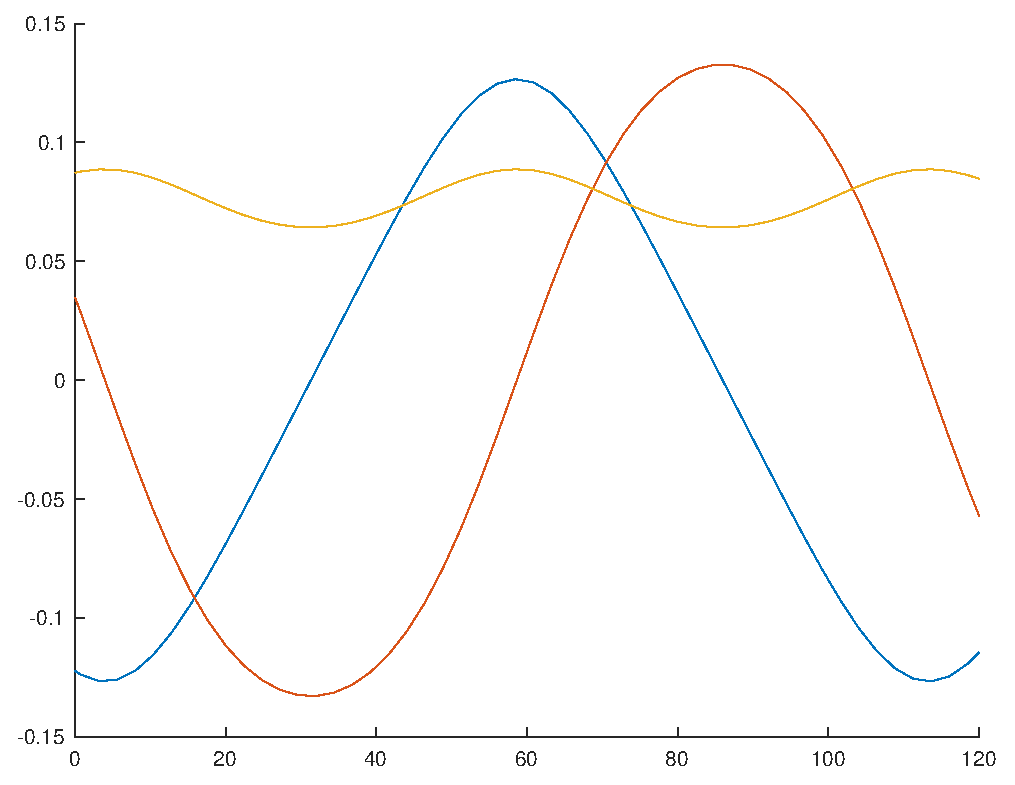
\includegraphics [width=4in]{HW2main_01.eps}

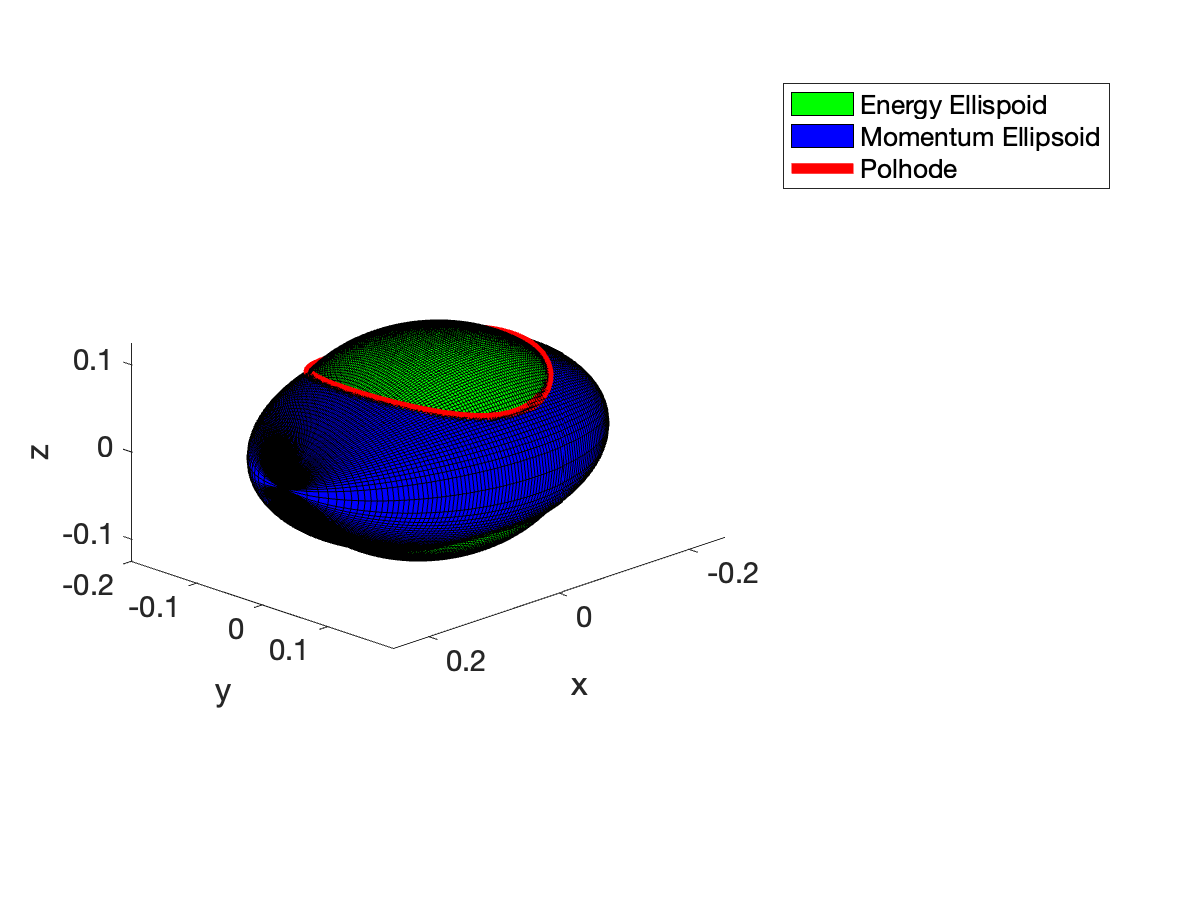
\includegraphics [width=4in]{HW2main_02.eps}

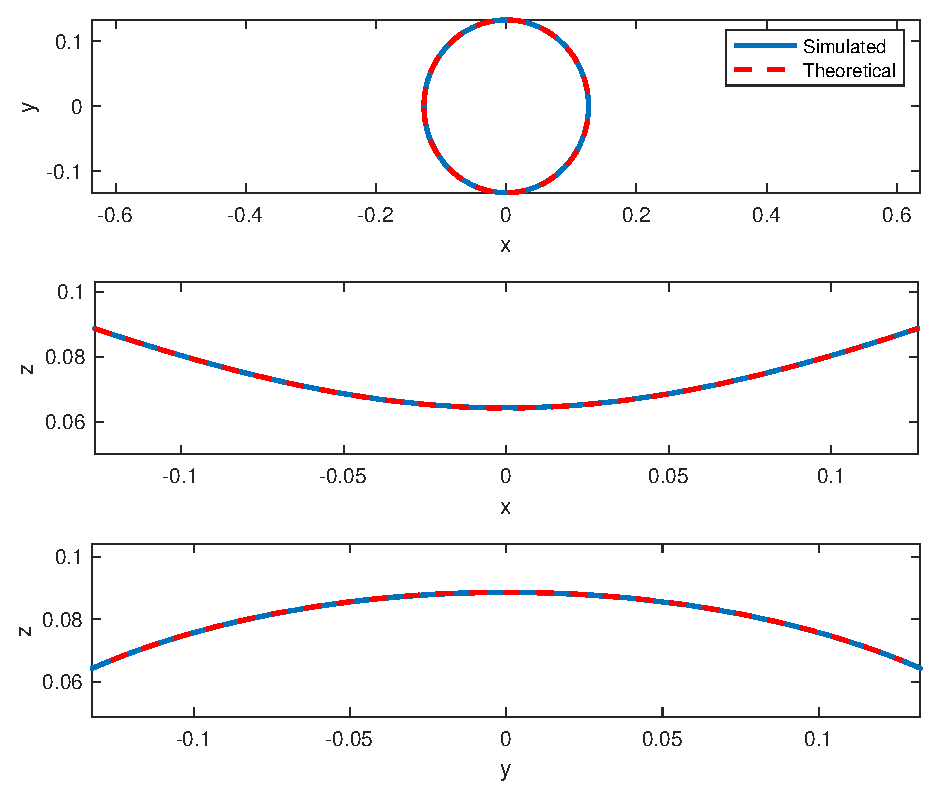
\includegraphics [width=4in]{HW2main_03.eps}

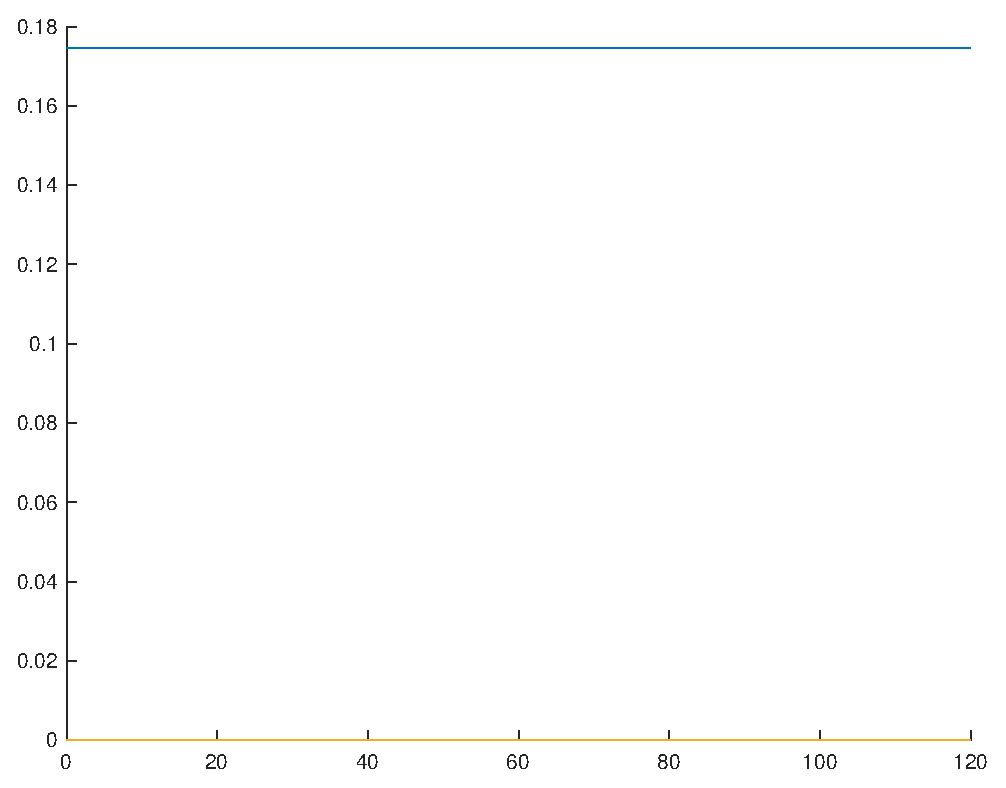
\includegraphics [width=4in]{HW2main_04.eps}

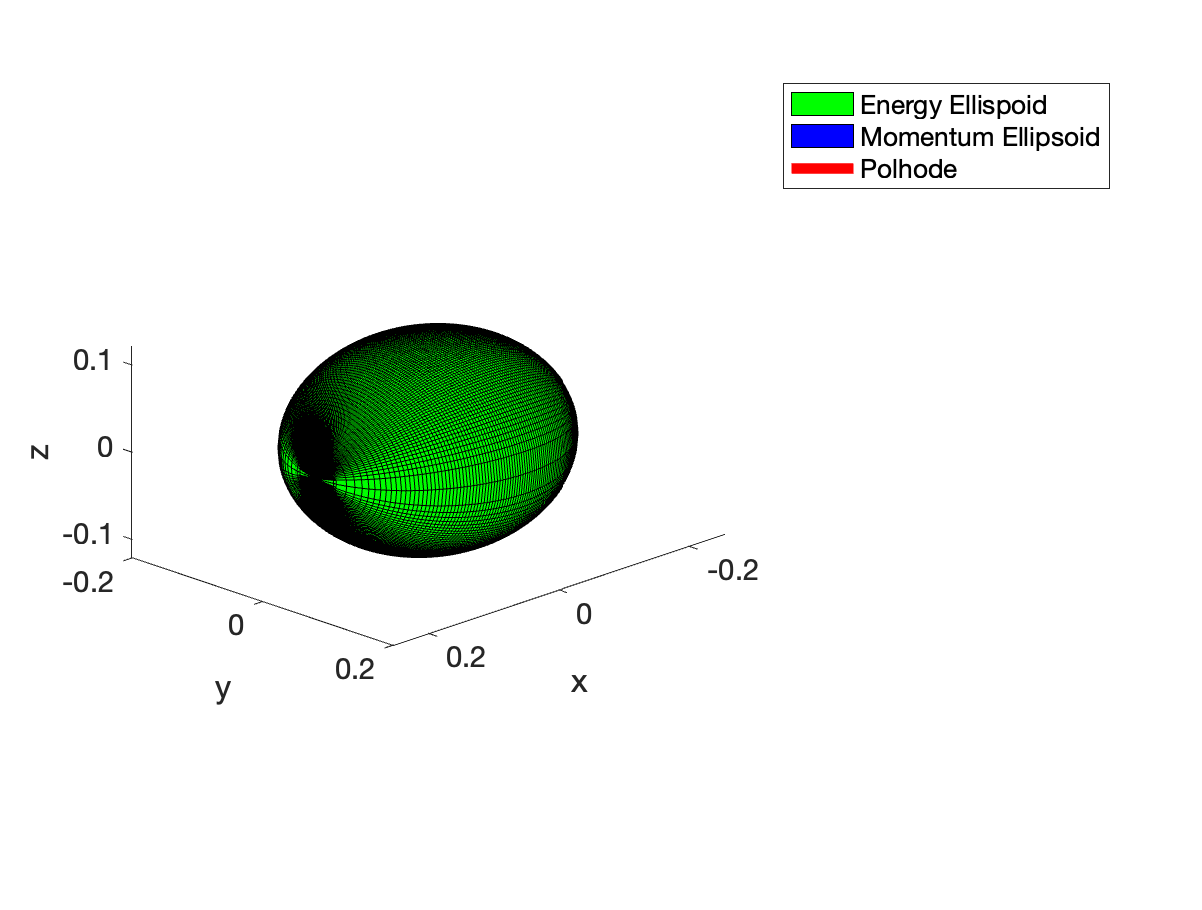
\includegraphics [width=4in]{HW2main_05.eps}

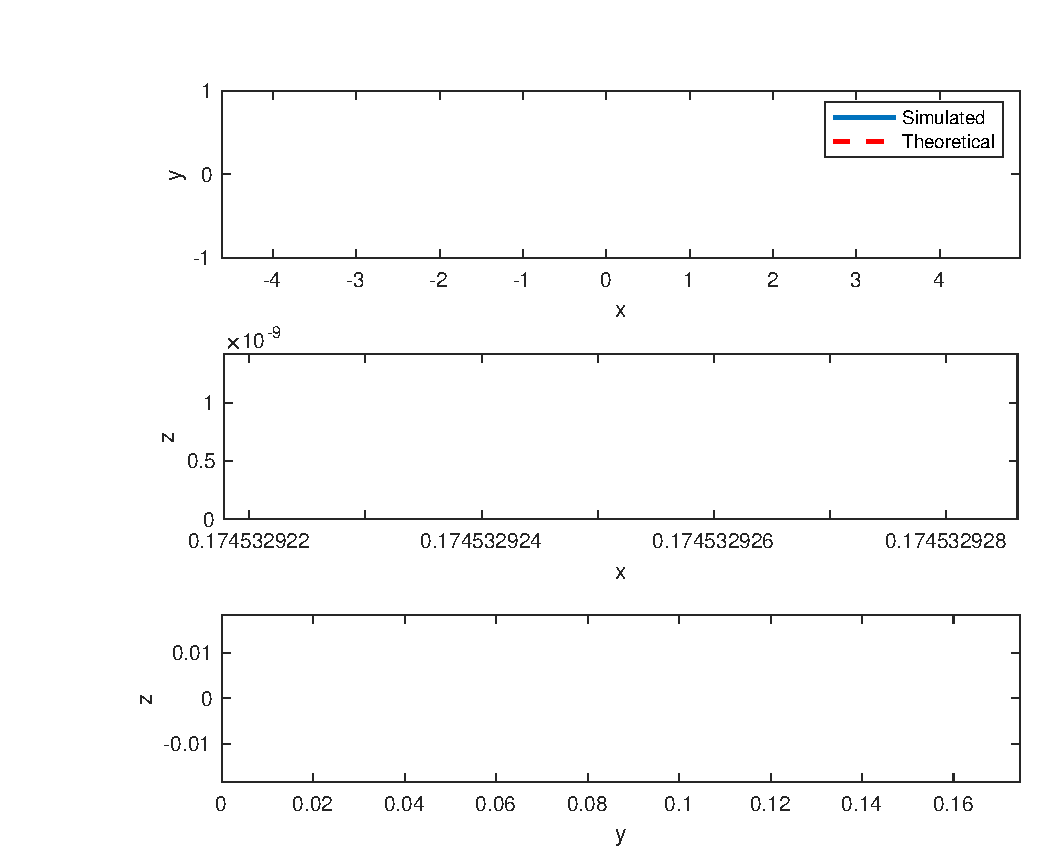
\includegraphics [width=4in]{HW2main_06.eps}



\end{document}

